\chapter{Anthropic Claude Code}

\section{Engineering principles}

Claude Code provides interactive and print-mode CLI execution, configuration scopes, reusable skills, MCP tools, event hooks and subagents. Project memory and persistent learning are distinct from security enforcement. The permission mode determines how tool requests are handled; the Bash sandbox addresses a separate execution boundary. A subagent can specialize on investigation or review, but independent validation still requires a separately controlled verifier.\src{A1,A2,A3,A4,A5,A6,A7,A8,A10}

\section{Implementation approach}

Install and authenticate through the official quickstart for the target operating system. Record \texttt{claude -{}-version} and \texttt{claude -{}-help}. Use a project CLAUDE.md that imports the shared AGENTS.md to avoid duplication. Start with plan mode to inspect a task, then use an approved write-capable configuration for implementation. The sample adapter uses print mode with dontAsk so unapproved actions fail rather than prompting an unattended process. Explicitly authorize only necessary operations in the managed environment.

\section{Verification and limitations}

Verify that permissions, hooks and sandbox prerequisites are effective. A shell restriction is not a complete isolation model for all tools; restrict the host, egress, credentials and MCP scopes independently. Do not enable bypass modes to make automation succeed.

Figure~\ref{fig:d4} illustrates the conceptual flow from Engineer / CLI to Workspace. The edges describe the proposed integration or control relationship, not undocumented internal calls.

\begin{figure}[htbp]\centering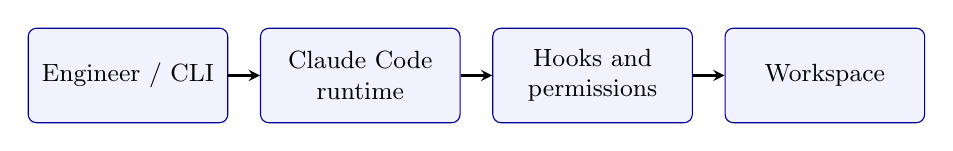
\begin{tikzpicture}[nodebox/.style={draw=blue!60!black,fill=blue!5,rounded corners=3pt,minimum height=12mm,text width=23mm,align=center,font=\small},>=stealth]
\node[nodebox] (n0) at (0.00,0.00) {Engineer / CLI};
\node[nodebox] (n1) at (2.95,0.00) {Claude Code runtime};
\node[nodebox] (n2) at (5.90,0.00) {Hooks and permissions};
\node[nodebox] (n3) at (8.85,0.00) {Workspace};
\draw[->,thick] (n0.east) -- (n1.west);
\draw[->,thick] (n1.east) -- (n2.west);
\draw[->,thick] (n2.east) -- (n3.west);
\end{tikzpicture}
\caption{Claude Code conceptual integration (conceptual view).}\label{fig:d4}\end{figure}

\section{Chapter conclusion}

Apply the stated verification criteria before expanding the scope of this workflow. Record deviations, evidence and unresolved risks in the task record.
